\chapter{Literature Review}
\label{ch:lit-review}

Commercial wireless power transfer technologies have developed as a response to both the ubiquity of mobile devices and limitations in traditional wired power. These technologies differ in range, efficacy, and method, but suggest an overall attempt to shift away from traditional charging mechanisms. This literature review will focus on the distinct methods that make up the current state-of-the-art of wireless power. These methods and companies are not meant to be exhaustive, but should be recognized as a quick overview toward these liminal technologies. This review will additionally explore WPT technologies based on their applicable ranges.

At the conclusion of this overview of the state-of-the-art in WPT, we will discuss both the general operation of time reversal and the historical developments of that field. This will include the acoustical roots of TR by Claire Prada and Matthias Fink, later communication accomplishments by Steven Anlage, and TESLA's modern WPT application.

\section{Wireless Power Transfer Vocabulary}

Several groups have already made practical WPT technologies. In this paper Powermat, WiTricity, Wattup, uBeam, Cota, and Wicharge will be considered as the state-of-the-art WPT methods. The technologies these companies use in their products will be compared using several different metrics, defined below. The capabilities of these technologies under these metrics are summarized in Table~\ref{tab:lit-review-company-compare}, and discussed in detail in the following sections. These companies represent many of the major players in the current WPT industry that either currently have a product on the market, are in the process of commericalizing a product, or have plans to commercialize a product in the next few years.

\def\arraystretch{2}
\begin{table}[t]
\centering
\begin{tabular}{|c|c|c|c|}
\hline
\textbf{Company} & \cellstack{\textbf{Method of}\\\textbf{Power Transfer}} & \cellstack{\textbf{Max Power}\\\textbf{Delivered (W)}} & \textbf{Approx. Range (ft.)} \\ \hline
Cota & \cellstack{Concentrated Microwaves} & 1 & 30 \\ \hline
Powermat & Inductive Coupling & 5 to 50 & Touching \\ \hline
uBeam & Ultrasound & \cellstack{Unknown\\(minimum 1.5)} & 3 to 13 \\ \hline
WattUp & RF & 10 & 15 \\ \hline
Wi-Charge & Laser & 10 & 30 \\ \hline
WiTricity & \cellstack{Resonant Inductive\\Coupling} & \cellstack{Scalable, on the\\order of 1000} & 7 \\ \hline
\end{tabular}
\caption[Comparison of wireless technology companies and their products' capabilities]{Comparison chart of wireless technology companies and their products' capabilities. The information in this table reflects publicly disclosed information at the time of writing.}
\label{tab:lit-review-company-compare}
\end{table}

As can be seen, the different WPT technologies vary wildly in both their methods of operation and their intended application. Comparing different WPT technologies is difficult because the measures of characterizing performance used in Table~\ref{tab:lit-review-company-compare} are poorly defined. The field of WPT lacks one central governing body that defines such performance metrics. This, combined with the constant battle for market prominence leads to many crucial details being withheld due to Intellectual Property (IP) rights. Because of this, we will specify our own definitions of performance metrics important to this thesis.

\subsection{Efficiency}

Efficiency in particular is difficult to quantify, as there does not currently exist a standardized definition used by all parties. In the literature, efficiency of transfer has included:
\begin{itemize}
    \item the amount of power delivered to the target compared to the amount of power drawn by the transmitter
    \item the transfer between antennas within a setup, with other losses (such as those due to rectifiers after transmission) being ignored
\end{itemize}

Here, the team defines efficiency as the amount of power delivered to the battery of the target device compared to the amount of electrical power input into the transmitter. We colloquially refer to this metric as ``wall to load'' efficiency.

The average efficiency of a corded phone chargers across eleven varieties of authentic, non-counterfeit chargers was found to be 72.4\%~\cite{sherriff2012}.

\subsection{Maximum Power}

The maximum amount of power that can be transmitted to a target using a given technology. Typically, this value is cited at relatively short distances, much shorter than the advertised ``maximum'' range. It should be specifically noted that there is generally a tradeoff between maximum power and range that is unavoidable.

Maximum power limits the devices that can be powered by a given technology. While high power transmission is not important for all devices, a larger range of power improves the flexibility of the technology.

\subsection{Active or Passive Transmission}

Some technologies require the device being powered to actively participate in the powering process, usually by broadcasting a signal to the WPT transmitter. We call this active transmission. Others, like charging mats, are ``always on'' as long as the device to be powered is within range: from the device's point of view, this is passive transmission. This can be important because active charging requires the device to expend power while passive can accommodate a completely dead device.

\section{Health Concerns}

Another topic that needs to be considered is the health effects (if any) on living creatures in the range of a WPT technology. Electromagnetic radiation is known to have potentially harmful effects to biological tissue at sufficiently large power density levels~\cite{adey1993biological}. The benchmark that is used to measure the applied power density that is transmitted to a person's skin is referred to as Specific Absorption Rating (SAR), which is a measure of the power deposited per unit mass of a material. In this case, the material is skin tissue and the SAR value is averaged over the entire body to arrive at a final value. In the US, the FCC legal limit on SAR is 1.6 $W/kg$~\cite{procon2015}. As a reference, the iPhone 5 has a cited SAR value of 1.18 $W/kg$~\cite{procon2015}. It is generally accepted that cell phone use is safe. As long as our TR process does not exceed the 1.6 $W/kg$ value, then we may assume it will be safe for human use and we do not need to be concerned with biological harm, as the FCC deems this a safe level of electromagnetic radiation.

\section{Overview of WPT Technologies by Company}
\label{sec:lit-review-tech}
In order to classify the different companies, we have divided them by advertised range. For the purposes of this discussion, we note 3 ranges: (1) very short range (up to 1 foot), (2) medium range (max of 15 feet), and (3) long range (max of 30 feet). Now that we have defined a basic classification system for the current WPT technologies we may proceed to a more in-depth discussion of the companies themselves.

\subsection{Very Short Range}
\subsubsection{Powermat}
The most restrictive technology in terms of range is that of Powermat. Devices are charged by being placed on the charging mat. Harnessing inductive coupling, the same method used to charge electric toothbrushes, Powermat has virtually no charging range, as the device and the charger must be in full contact. The technology is capable of charging multiple devices, but the system requires compatibility devices for any that are not already Powermat-enabled off-the-shelf.

As the charging mat is wired, its range is still restricted to the length of a power cord. If the device is not compliant with the Powermat standard, then it must be plugged into a compatibility device anyway. That said, the mat can deliver between 5W and 50W, making it a very effective charging tool. Powermat compatible devices can be made without any external plugs, which could be desirable for applications such as waterproofing. Another interesting application has been the implementation of PowerMat devices inside furniture \cite{rogercheng205}. This allows tabletops to be transformed into charging surfaces.

\subsection{Medium Range}

\subsubsection{WiTricity}
Boston-based company WiTricity has expanded the previously discussed magnetic induction using a method they call highly resonant magnetic coupling (HRMC). Whereas traditional magnetic induction operates on the order of centimeters, HRMC is applicable at the meter scale. WiTricity reports 50\% efficiency at two meters, followed by 10\% efficiency at four meters~\cite{kesler_highly_2013,tucker_contribution_2013}. HRMC has charged multiple devices without seemingly sacrificing overall efficiency~\cite{kesler_highly_2013}. The public demonstrations by WiTricity show that HRMC can transmit power ranging from milliwatts to kilowatts, significantly more than was practical with traditional induction~\cite{kesler_highly_2013}.

\begin{figure}[t]
\centering
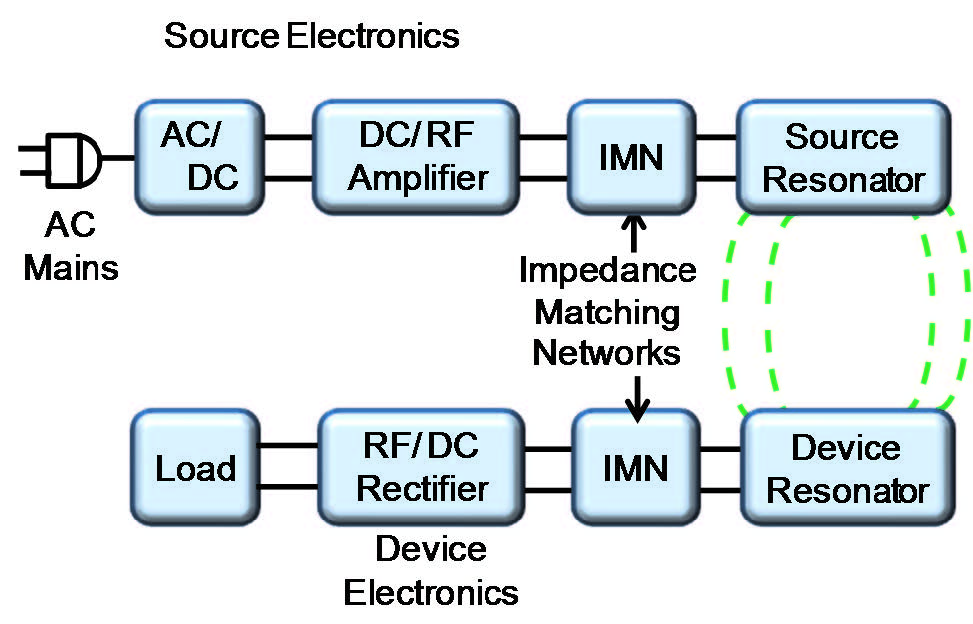
\includegraphics[width=0.85\textwidth]{lit-review/witricity-schematic}
    \caption[WiTricity schematic]{Schematic of WiTricity's HRMC System~\cite{kesler_highly_2013}}
    \label{fig:lit-review-witricity-schematic}
\end{figure}

HRMC uses magnetic induction to transmit energy between two coupled antennas. HRMC continually adjusts the coupling of transmitter and receiver antennas to keep both at a mutual resonant frequency. This technique, impedance matching, minimizes the amount of wave reflection inside the transmitter and receiver circuits, maximizing the power passed to the load component. This process requires a continuous proprietary feedback mechanism to optimize the receiver for the given distance from the transmitter.

WiTricity has demonstrated that the range of HRMC can be increased through the use of coupled relays. These relays can be coupled with the transmitter, allowing the effective range of the transmitter to increase with minimal additional loss~\cite{butler_tour_2013}.

\subsubsection{WattUp}
WattUp's central idea is to use Bluetooth to transfer information about the receiver's location relative to the transmitter, allowing the transmitter to directly focus energy on the receiver~\cite{energouscorporation2016}. Once it has locked in a signal, it may boost the output power from mW RF signals to multiple W RF signals such that the receiver can charge. WattUp highlights two main features of its technology: (1) the range over which \numrange{1}{4}~W may be quickly and safely transmitted and (2) the relatively large number of devices that may be powered at once (currently 12, with 24 being available in the future)~\cite{energouscorporation2016}.

WattUp cites that they may deliver up to 4~W to 4 devices simultaneously within 0-5 feet of the transmitter, 2~W to 4 devices simultaneously within \numrange{5}{10}~feet, and 1~W within \numrange{10}{15}~feet~\cite{energouscorporation2016}. This inverse relationship between delivered power and range is similar to the trend seen with WiTricity, as previously discussed. These numbers only represent the current model and demonstration version of the technology. WattUp claims that for ranges up to 5 feet, the device will charge as if it were plugged into a wall outlet, for 5-10 feet, the device will resemble USB port charging from a computer, and for \numrange{10}{15}~feet users can still power up at slower charge rates. Based on the aforementioned values provided by WattUp, the overall max range is about 15 feet with a max output power of about 10 W, although these two conditions may not be met at the same time.

The technology itself uses two separate RF frequencies to perform wireless charging, representing both the Bluetooth communication (2.4~GHz) and power transfer frequency (5.7~GHz)~\cite{energouscorporation2016}. Both of these frequencies are allowed unlicensed frequency bands that are known to be used for wireless communication. We believe that WattUp chose to use separate frequencies in order to more easily differentiate the signals used for either targeting or power transfer. As the targeting algorithm is proprietary, we are unable to comment on their exact methodology for targeting the receiver.

\subsubsection{uBeam}
The final primary medium range WPT technology, titled uBeam, uses an entirely unique method compared to other companies and methods, relying on ultrasonic waves rather than electromagnetic waves~\cite{constine_ubeam_2015}. One can imagine their system as an extremely high power microphone and speaker combination that specifically sends the sound to a device location. Although uBeam is unique in its approach, it boasts comparable range and power levels when discussed next to other WPT companies.

The first difficulty of using sound waves as opposed  to electromagnetic waves is the inherent dissipative nature of air as a medium. Due to this characteristic, uBeam uses output sound levels of \numrange{145}{155}~dB (316 - 3000~$\frac{W}{m^2}$), comparable to the sound produced by a jet engine or shotgun blast ~\cite{galencarolaudio207}. In order for this level of sound to be used safely, uBeam uses transmission frequencies of \numrange{45}{75}~kHz, as this is far above the audible range of both humans and animals. As an extra safety measure, uBeam cites that ``if a person were to be exposed to the uBeam ultrasound source, 99.9\% of the emitted ultrasound will bounce off the skin''~\cite{constine_ubeam_2015}. These considerations have allowed uBeam to stay well within the FCC safety regulations.
uBeam uses a phased array transmitter with thousands of antennas that result in a power range of \numrange{1}{4}~m. Although the tracking and targeting algorithm is proprietary in nature, uBeam claims the ability to maintain power transfer while the receiver is moving, although uBeam does not cite specific speeds. The technology requires few obstructions in order to work due to the nature of sound as a mechanical oscillation. For example, if a cell phone is in a user's pocket, then it will not be able to be powered, as the user's clothing will block or extremely dampen the ultrasonic waves.

As their product has not yet hit the market, numbers for uBeam's efficiency are not available. We do know that the power output from the transmitter is \numrange{145}{155}~dB ~\cite{constine_ubeam_2015}, while a reasonable output at the receiver is on the order of \numrange{1}{10}~ watts. Based on this, the technique seems unlikely to have a high wall-to-load efficiency.

\subsection{Long Range}

\subsubsection{Cota}

Cota\textsuperscript{TM} by Ossia uses phase conjugation of a continuous microwave signal in order to focus energy at a precise location. While this is a very similar concept to the time reversal process we will describe in the rest of this thesis, here phase conjugation is operated at a single frequency, compared to our time reversal process, which uses a wider bandwidth. The basic idea of phase conjugation is exemplified in Figure~\ref{fig:lit-review-phase-conj}.

\begin{figure}
\centering
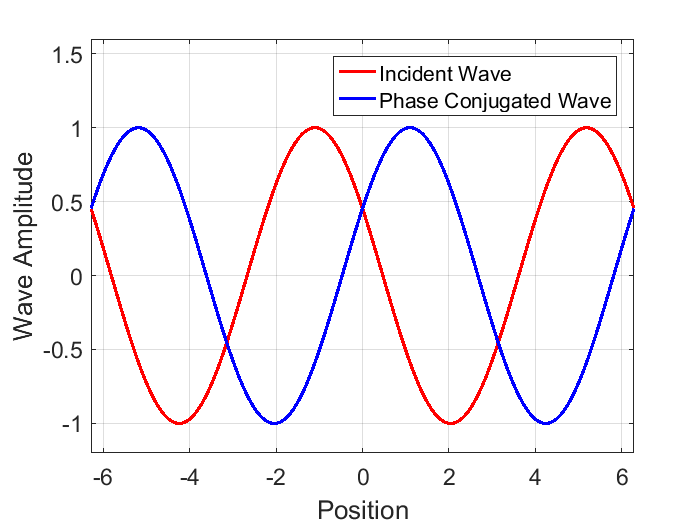
\includegraphics[width=0.85\textwidth]{lit-review/phase_conjugation}
    \caption[Phase Conjugation Example]{An initial incident wave received by a phase conjugate mirror and the corresponding phase conjugate reflected by the mirror. The phase conjugate wave is, unsurprisingly, a phase-shifted version (in this case offset by $\pi$) of the incident wave.}
    \label{fig:lit-review-phase-conj}
\end{figure}

The current iteration of the Cota system at the time of writing consists of two components: a base station with a large array of 1,000 to 8,000 transmitting micro-antennas and a receiver device. The receiver device initiates the power transfer process by sending out a low power omni-directional beacon pulse 100 times per second, as shown in Figure~\ref{fig:lit-review-cota-example}(a), which propagates throughout the room, reflecting off walls, and eventually being recorded by the transmitter. The transmitter then calculates the ``complex conjugate'' of each wave recorded and transmits this mirror image of each wave, as shown in Figure~\ref{fig:lit-review-cota-example}(b), which ultimately converge at the receiver to deliver power~\cite{cota-handout}. Since the initial pulse is omni-directional, some waves will of course end up hitting obstacles, such as people. However, the low power of this pulse makes them harmless, and the obstruction of the wave itself prevents this wave from reaching the transmitter, meaning that a higher power reflection will not make it back to the obstruction, and thus the technology naturally avoids obstacles. Since the position of the beacon is recalculated 100 times per second, they claim to be able to provide power to moving devices. The transmitter continually sweeps through a variety of frequencies in attempt to find the best $S_{21}$ parameter between the antenna and beacon. Even once it has settled on a frequency it continues this sweep and adjusts the frequency as the channel conditions change if necessary.

\begin{figure}
\centering
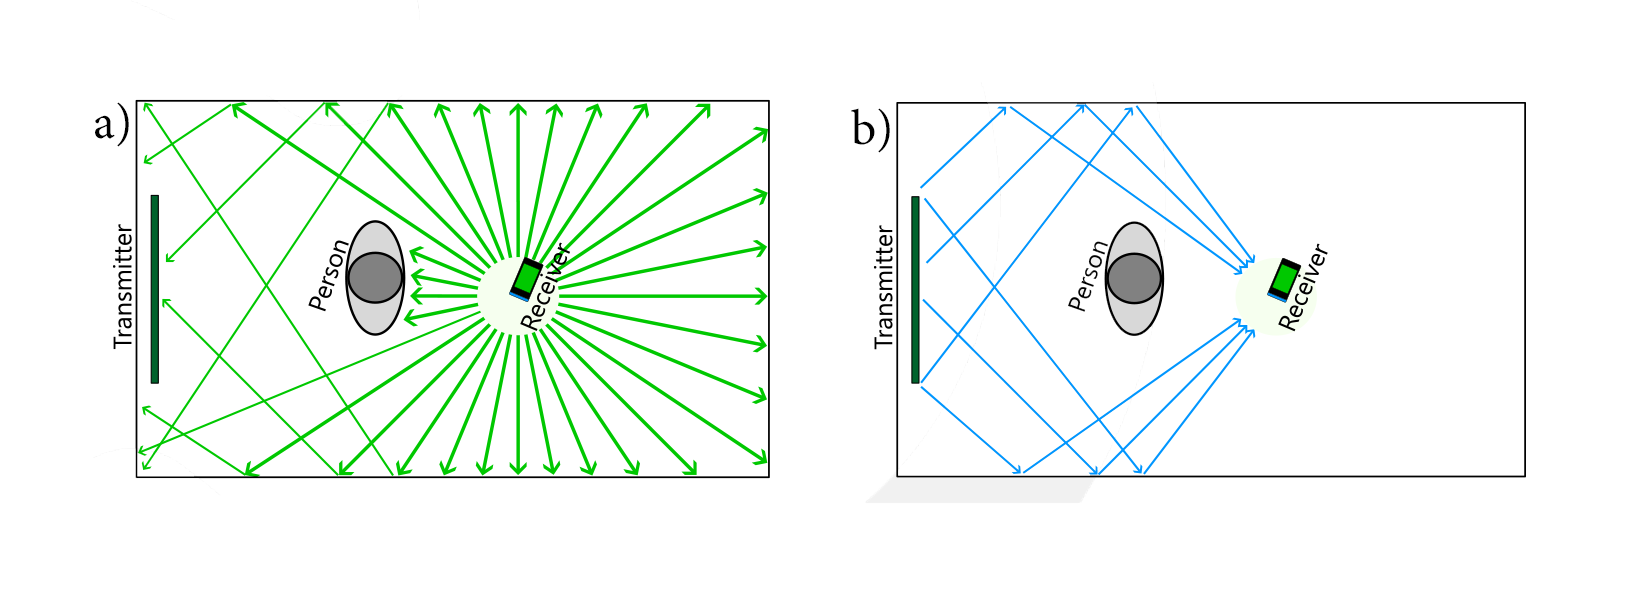
\includegraphics[width=0.85\textwidth]{lit-review/cota_example}
    \caption[Cota Process]{Description of the basic Cota power transfer protocol, which utilizes ``multi-path'' trajectories to avoid obstructions, as opposed to a ``beam forming'' power transfer system.}
    \label{fig:lit-review-cota-example}
\end{figure}

Cota's use of a single frequency simplifies the process because it means they only have to adjust the phase of the oscillator driving each antenna in the array. In addition, it allows them to work peacefully in a small pocket of the 2.4~GHz ISM band, without interfering with the majority of the spectrum that is utilized by Wi-Fi devices. In addition, Zeine claims that lower frequencies have longer wavelengths that preclude the formation of ``small'' pockets of energy, while higher frequencies (such as 24~GHz) have much more stringent SAR limits set by the FCC.

Although many press releases about Cota claim that it can deiver up to 1 Watt of power at up to 10 meters, Zeine admitted that this was a goal, and not yet an achieved result (they are able to transmit up to 1 Watt of power, but only at unspecified ``shorter'' distances). They also were not able cite specific efficiency numbers, but admitted that they were ``not high''. The beacon currently broadcasts 24~dBm at 100~Hz, and the base station emits 5-10~W of power.

\begin{figure}
\centering
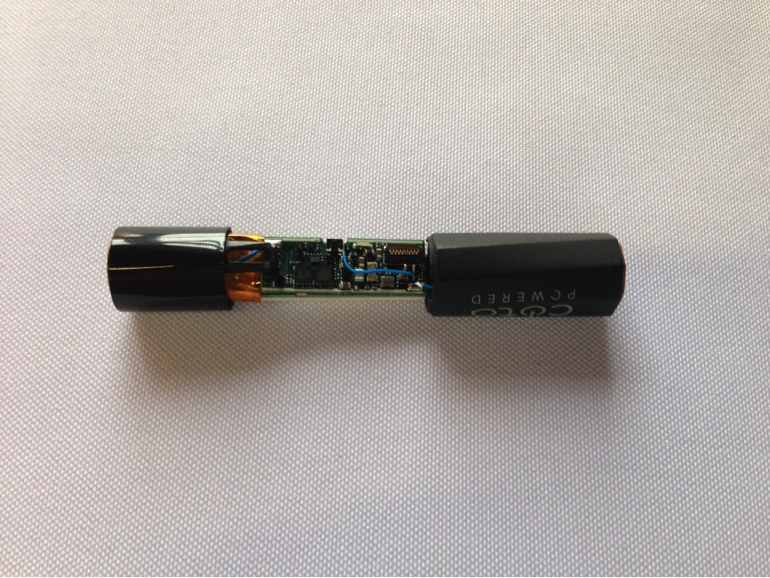
\includegraphics[width=0.85\textwidth]{lit-review/cota_battery}
    \caption[Cota Battery]{This photo of a Cota ``AA Battery'' was taken at the Ossia/Cota demonstration table at IEEE WPTC 2016. The technical representative stated that the battery constantly tops off power from the base station and stores this in a buffer until it is used by the device.}
    \label{fig:lit-review-cota-battery}
\end{figure}

However, Cota has a grand vision for the improvement of these numbers and ultimately the incorporation of their technology into all of our mobile devices and the emerging set of ``Internet of Things'' devices. They already have created phone cases that can be attached to a typical mobile phone allowing existing devices to act as Cota receivers, though they ultimately envision that future devices will have Cota receivers built in. In addition, they have created ``AA Batteries'' (shown in Figure~\ref{fig:lit-review-cota-battery}) that house the entire Cota receiver system, which both exemplifies how small the receiving circuit can be, and also allows Cota to retrofit the vast array of devices that currently rely on batteries without any modifications to the device. Zeine claims that they are currently working with paint and carpet manufacturers to make their products more conductive, which would provide better reflections for power transmission.

It is worth noting that, at the time of writing, Ossia has not yet released any peer-reviewed publications or white papers detailing the Cota technology. The information above was compiled from Ossia's ``Wireless power transfer system patents''~\cite{cota-patent} and conversations with Ossia's CEO, Hatem Zeine, at the 2016 IEEE Wireless Power Transfer Conference in Aveiro, Portugal.

\subsubsection{Wi-Charge}

\begin{figure}
\centering
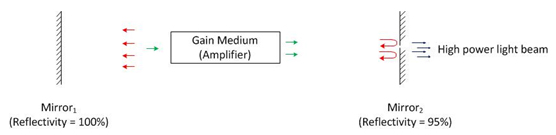
\includegraphics[width=0.85\textwidth]{lit-review/wicharge-1}
    \caption[Wi-Charge: Typical laser]{The resonating chamber of a typical laser. The gain medium allows for stimualted emission of photons. The 95\% reflective mirror partially transmits light, which is observed as the output of the laser~\cite{wicharge2016}.}
    \label{fig:lit-review-wicharge-1}

\vspace*{\floatsep}% http://tex.stackexchange.com/q/26521/5764

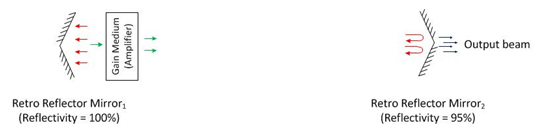
\includegraphics[width=0.85\textwidth]{lit-review/wicharge-2}
    \caption[Wi-Charge: Modified resonating cavity]{A modification of the traditional laser resonating cavity to allow for collimation and coherency of the stimulated photons~\cite{wicharge2016}.}
    \label{fig:lit-review-wicharge-2}

\vspace*{\floatsep}% http://tex.stackexchange.com/q/26521/5764

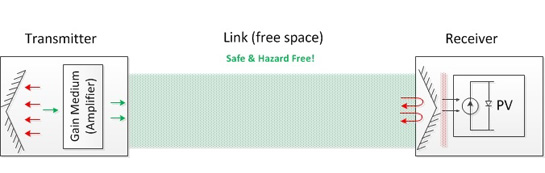
\includegraphics[width=0.85\textwidth]{lit-review/wicharge-3}
    \caption[Wi-Charge: Wi-Charge setup]{The setup of the Wi-Charge system. The fully reflective mirror is on the transmitter, while the 95\% reflective mirror is located within the receiver device. Behind the receiver's mirror is a photovoltaic cell to convert the light back into an electrical signal to power a battery~\cite{wicharge2016}.}
    \label{fig:lit-review-wicharge-3}
\end{figure}

Also capable of a 30~ft operating radius, Wi-Charge uses a combination of a laser cavity and a photovoltaic cell to create robust power transfer systems~\cite{wicharge2016}. To understand the system, it is necessary to discuss how a laser works. Consider Figure~\ref{fig:lit-review-wicharge-1}, which depicts two mirrors and an amplifier between them. Simply put, one photon, an energetic light particle, enters the amplifier and two come out. When the photons hit the mirror, they bounce back through the amplifier in the opposite direction and two photons become four. This process repeats with each ricochet against a mirror, and the energy amplifies within the system. This process of recirculating light in a positive feedback loop with an amplifier creates a resonator.

When that resonator has one mirror that is very slightly transparent, as in Figure~\ref{fig:lit-review-wicharge-1}, then a focused, high powered beam is generated. This is a laser beam.

Any particles that do not travel along the axis between the two mirrors will hit the mirror at an odd angle and bounce out of the resonator. This is why only the photons that are traveling in the direction of the axis between the two mirrors will continue to amplify.

Wi-Charge took this traditional definition of a laser, and made a few clever modifications to better suit their purposes, shown in Figure~\ref{fig:lit-review-wicharge-2}~\cite{wicharge2016}.

First, they kept the components--two mirrors with an amplifier between them--but modified their arrangement. Second, they made the mirrors retro-reflectors which, unlike regular mirrors, reflect light back to their sources. The result is that the two mirrors spontaneously form a resonator when placed within each other's \los{}, although the resonator is stalled immediately when the \los{} is broken. This last property may actually be desireable in a consumer setting, as it helps to prevent energy from accumulating anywhere but the intended receiver.

In Wi-Charge's setup, one mirror and the amplifier are grouped together as the transmitter, and a second mirror and a photovoltaic cell are grouped together as the receiver. This is shown in Figure~\ref{fig:lit-review-wicharge-3}. By placing the photovoltaic cell directly after the laser output location, the Wi-Charge system effectively converts the optical signal back to an electrical signal that can be used to charge a battery.

Wi-Charge is a long range wireless power solution that can deliver up to 10~W of power~\cite{wicharge2016}. It can latch onto targets almost instantaneously and cease beaming equally quickly, intrinsically. It can also power multiple devices. However, the system does require \los{}.

\section{Time Reversal}
\label{lit-review-tr}

\subsection{Conceptual Overview of Time Reversal}

The lossless wave equation is time-reversal invariant: for any normally propagating wave taken to be a time-forward solution, there is a corresponding time-reversed solution representing that wave traveling in the opposite direction. The technique known as time reversal (TR) exploits this property of waves to focus a signal onto the point of origin of some other, previous signal. TR can locate objects without prior knowledge of their position or their surrounding geometry.

A system that performs TR is called a ``time reversal mirror'' (TRM), sometimes simply shortened to ``mirror.'' A TRM consists of one or more transmitters to introduce waves into a chamber and one or more receivers to record the echoes from it. The transmitters and receivers may (but do not have to be) the same device. TR requires an at least partially echoic chamber that allows waves to reflect off of its interior geometry and return to the transmitters. Here we refer to such a chamber as ``reverberant''.

\begin{figure}
    \centering
    \begin{subfigure}{.85\textwidth}
        \centering
        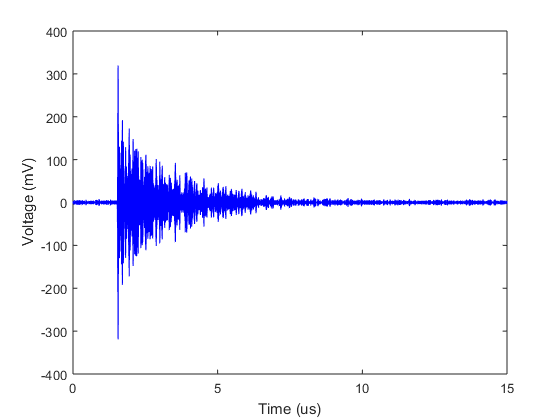
\includegraphics[width=0.9\linewidth]{lit-review/example-sona}
        \caption[Example sona]{Example sona}
         \label{fig:lit-review-example-sona}
    \end{subfigure}
		\par\bigskip
    \begin{subfigure}{.85\textwidth}
        \centering
        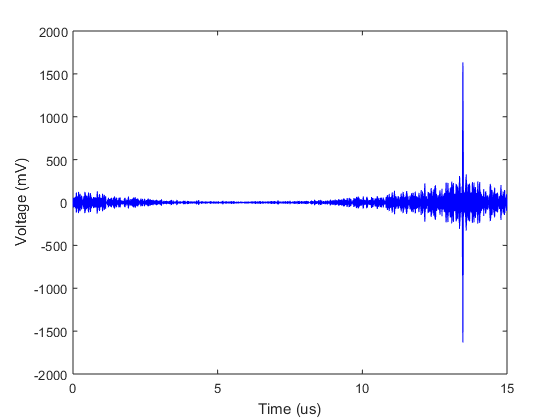
\includegraphics[width=0.9\linewidth]{lit-review/example-recon}
        \caption[Example reconstruction]{Example reconstruction}
         \label{fig:lit-review-example-recon}
    \end{subfigure}
    \caption{Recorded sona and reconstruction from a typical TRM experiment}
    \label{fig:lit-review-example}
\end{figure}

A TRM works by broadcasting a waveform into the reverberant chamber and recording the resultant echo. This echo will consist of many time-shifted overlays of the original waveform. We refer to this echo as a ``sona'' in this thesis. An example sona is shown in Figure~\ref{fig:lit-review-example-sona}. The sona is time reversed and rebroadcast, which will cause the waves to trace their paths in reverse and return to their source in a semi-coherent ``reconstruction'' of the original broadcast. An example reconstruction is shown in Figure~\ref{fig:lit-review-example-recon}: in this case, the original signal was a short pulse in the same shape as the large vertical spike near the right of the figure. Since it involves waves from many scattered paths all suddenly arriving at the same point, reconstruction is also known as ``collapse.''

TR is relatively versatile. If the technique is iterated exactly as described, the broadcasts will collapse more and more exactly on the strongest scatterer in the chamber~\cite{fink_time-reversed_1999}. Many other methods can be used to select targets more discriminately, and the generic TRM itself can be modified as well -- for example, by recording directly from a target position, it is possible to create a secure channel between that point and the transmitter~\cite{nltr-wave-chaotic}.

\subsection{History of Time Reversal Research}

TR is a proven technique in signal processing, with applications in acoustics as well as electromagnetics. Though its publicity is limited, there is a wealth of available literature regarding TR in certain specialized areas. Here we briefly describe the development and historical applications of the technique to illustrate where TESLA's project will expand this literature.

Time reversal as a technique was first developed in the 1990s. Some of the earliest and most influential work was conducted through teams led by Mathias Fink and Claire Prada of the University of Paris. These researchers used the technique to focus sound waves on ``scatterers,'' objects that reflect the pulses~\cite{prada_iterative_1991}. An array of transducers would fire a sonic pulse into some propagation medium and listen for the echo. The recording of that echo was reversed in the time domain and transmitted back into the medium. They repeated (iterated) this process, causing the acoustic signature of the strongest scatterer to appear more prominently each time. In this way, the team was able to iteratively focus on the scatterers without needing prior knowledge of their location. Prada and her team submitted this DORT (French acronym, English: Decomposition of the Time Reversal Operator) method as a process for finding cracks or faults in structural members~\cite{prada_iterative_1991}. More importantly, Prada et al. went on to demonstrate that the method could always resolve the brightest scatterer if given enough iterations, that it worked better in a heterogeneous medium than a homogenous one, and that it was both experimentally and mathematically possible to resolve multiple targets at once~\cite{prada_decomposition_1996}. These discoveries generated significant interest in a subset of the acoustics research community.

Others in the field of acoustics went on to refine the DORT method as an imaging technique, and as the field gathered attention, further explored formalizing the problem in general. An excellent example of the latter is the theoretical work by D. H. Chamber in his 2007 examination of TR for target detection and characterization~\cite{chambers_target_2007}. In 2010, Nguyen and Gan developed a way to extract much more information from an anisotropic (directionally distinct) scatterer, including its rough shape, density, and radius. In doing so, they developed a faster mathematical approach to locating their scatterers that relied on several good approximations instead of one exhaustive computation~\cite{nguyen_dort_2010}. Also in 2010, Barbieri and Meo made a large contribution to the field by bringing together the DORT method, which works in linear environments, and another similar method for working in nonlinear environments. This allowed them to resolve and distinguish between linear scatterers such as holes and nonlinear scatterers such as cracks~\cite{barbieri_time_2010}.

Imaging is not the only application for a focusing method, however, and others adapted the existing body of TR research to new problems. The reciprocity of the wave function that Fink and Prada relied on to develop the technique holds for all waves it can be used to model. This means that the time-reversal operation works much the same way with electromagnetic waves as it does with sound waves~\cite{chambers_target_2007}. This was explored as early as 1999, but was largely concerned with the same imaging problems occupying those in acoustics until at least 2007~\cite{chambers_target_2007}. However, that gradually began to change. In 2011, a team including graduate students from the University of Maryland posited that time reversal was an ideal mechanism for wireless communication~\cite{wang_green_2011}. In the same way that a sound wave could be made to collapse on a scatterer, they showed that an information packet could be made to collapse on a receiver. The team submitted this as an eco-friendly communication method because information transfer could be accomplished using less energy~\cite{wang_green_2011}. Later, this same property was examined for its security benefits instead of its environmental ones. In February of 2013, a team of researchers at the University of Maryland, including Matthew Frazier and Steven Anlage, published a study discussing TR as a method to selectively send information in a chaotic wave environment~\cite{nltr-wave-chaotic,taddese_sensing_2010}. The team was able to create an exclusive communication link to a certain object, without needing to know its location and without interfering with nearby objects. In their experiment, they were able to transmit data (in the form of images) exclusively to a desired port, while the other port received only garbled noise.

Beyond its practical applications, in the process, Frazier and his team used nonlinear elements to extend TR in new and exciting ways. Recall that in traditional TR many iterations are required to pinpoint the target. The addition of a significantly nonlinear element greatly simplifies the pinpointing process. When a wave strikes the element, harmonic frequencies are produced at integer multiples of the original frequency. These harmonics can be quickly located in the echo's frequency domain and filtered in order to select them exclusively. The important distinction is that since the harmonics originated directly from the target antenna, all subsequent broadcasts of the TR signal will collapse on the antenna without the need for iteration~\cite{nltr-wave-chaotic}. Frazier and the others put forth several exciting directions to pursue with this concept: the secure communication channels mentioned above, hyperthermic treatment of tumors, and a long range WPT system that eschews traditional high power beams. It is this last area that TESLA intends to explore.
